\documentclass[unicode,11pt,a4paper,oneside,numbers=endperiod,openany]{scrartcl}
\newcommand\tab[1][0.5cm]{\hspace*{#1}}
\usepackage{array}
\usepackage{multirow}
\usepackage{graphicx}
\usepackage[utf8]{inputenc}
\usepackage{listings}
\usepackage{xcolor}
\usepackage{seqsplit}
\usepackage{float}
\usepackage{booktabs}
\usepackage{subcaption}
\usepackage{adjustbox}
\usepackage{listings}
%New colors defined below
\definecolor{codegreen}{rgb}{0,0.6,0}
\definecolor{codegray}{rgb}{0.5,0.5,0.5}
\definecolor{codepurple}{rgb}{0.58,0,0.82}
\definecolor{backcolour}{rgb}{0.98,0.98,0.98}
%Code listing style named "mystyle"
\lstdefinestyle{mystyle}{
  backgroundcolor=\color{backcolour}, commentstyle=\color{codegreen},
  keywordstyle=\color{magenta},
  numberstyle=\tiny\color{codegray},
  stringstyle=\color{codepurple},
  basicstyle=\ttfamily\footnotesize,
  breakatwhitespace=false,         
  breaklines=true,                 
  captionpos=b,                    
  keepspaces=true,                 
  numbers=left,                    
  numbersep=5pt,                  
  showspaces=false,                
  showstringspaces=false,
  showtabs=false,                  
  tabsize=2,
  numbers=none
}
\lstdefinestyle{base}{
  language=C,
  emptylines=1,
  breaklines=true,
  basicstyle=\ttfamily\color{black},
  moredelim=**[is][\color{red}]{@}{@},
}
\lstset{style=mystyle}
\newcommand\MyBox[2]{
  \fbox{\lower0.75cm
    \vbox to 1.7cm{\vfil
      \hbox to 1.7cm{\hfil\parbox{1.4cm}{#1\\#2}\hfil}
      \vfil}%
  }%
}
\usepackage{ifthen}
\usepackage[utf8]{inputenc}
\usepackage{graphics}
\usepackage{graphicx}
\usepackage{hyperref}

\pagestyle{plain}
\voffset -5mm
\oddsidemargin  0mm
\evensidemargin -11mm
\marginparwidth 2cm
\marginparsep 0pt
\topmargin 0mm
\headheight 0pt
\headsep 0pt
\topskip 0pt        
\textheight 255mm
\textwidth 165mm

\newcommand{\duedate} {}
\newcommand{\setduedate}[1]{%
\renewcommand\duedate {Due date:~ #1}}
\newcommand\isassignment {false}
\newcommand{\setassignment}{\renewcommand\isassignment {true}}
\newcommand{\ifassignment}[1]{\ifthenelse{\boolean{\isassignment}}{#1}{}}
\newcommand{\ifnotassignment}[1]{\ifthenelse{\boolean{\isassignment}}{}{#1}}

\newcommand{\assignmentpolicy}{
\begin{table}[h]
\begin{center}
\scalebox{0.8} {%
\begin{tabular}{|p{0.02cm}p{16cm}|}
\hline
&\\
\multicolumn{2}{|c|}{\Large\textbf{HPC  2022 ---  Submission Instructions}}\\
\multicolumn{2}{|c|}{\large\textbf{(Please, notice that following instructions are mandatory: }}\\
\multicolumn{2}{|c|}{\large\textbf{submissions that don't comply with, won't be considered)}}\\
&\\
\textbullet & Assignments must be submitted to \href{https://www.icorsi.ch/course/view.php?id=14652}{iCorsi} (i.e. in electronic format).\\
\textbullet & Provide both executable package and sources (e.g. C/C++ files, Matlab). 
If you are using libraries, please add them in the file. Sources must be organized in directories called:\\
\multicolumn{2}{|c|}{\textit{Project\_number\_lastname\_firstname}}\\
& and  the  file must be called:\\
\multicolumn{2}{|c|}{\textit{project\_number\_lastname\_firstname.zip}}\\
\multicolumn{2}{|c|}{\textit{project\_number\_lastname\_firstname.pdf}}\\
\textbullet &  The TAs will grade your project by reviewing your project write-up, and looking at the implementation 
                 you attempted, and benchmarking your code's performance.\\

\textbullet & You are allowed to discuss all questions with anyone you like; however: (i) your submission must list anyone you discussed problems with and (ii) you must write up your submission independently.\\
\hline
\end{tabular}
}
\end{center}
\end{table}
}
\newcommand{\punkte}[1]{\hspace{1ex}\emph{\mdseries\hfill(#1~\ifcase#1{Points}\or{Points}\else{Points}\fi)}}


\newcommand\serieheader[6]{
\thispagestyle{empty}%
\begin{flushleft}

\includegraphics[width=0.4\textwidth]{images/usi_inf.png}
\end{flushleft}
  \noindent%
  {\large\ignorespaces{\textbf{#1}}\hspace{\fill}\ignorespaces{ \textbf{#2}}}\\ \\%
  {\large\ignorespaces #3 \hspace{\fill}\ignorespaces #4}\\
  \noindent%
  \bigskip
  \hrule\par\bigskip\noindent%
  \bigskip {\ignorespaces {\Large{\textbf{#5}}}
  \hspace{\fill}\ignorespaces \large \ifthenelse{\boolean{\isassignment}}{\duedate}{#6}}
  \hrule\par\bigskip\noindent%  \linebreak
 }

\makeatletter
\def\enumerateMod{\ifnum \@enumdepth >3 \@toodeep\else
      \advance\@enumdepth \@ne
      \edef\@enumctr{enum\romannumeral\the\@enumdepth}\list
      {\csname label\@enumctr\endcsname}{\usecounter
        {\@enumctr}%%%? the following differs from "enumerate"
	\topsep0pt%
	\partopsep0pt%
	\itemsep0pt%
	\def\makelabel##1{\hss\llap{##1}}}\fi}
\let\endenumerateMod =\endlist
\makeatother




\usepackage{textcomp}






\usepackage{subcaption}

\begin{document}


\setassignment

\serieheader{Security ML}{2023}{Student: Filippo Casari}{}{Report for Assignment 2}{}
\newline
\section{Malware Detection}


\subsection{Understanding the Data}
First, I would say that a lot of features are important to detect a malware in an Android application since certain permissions or using some APIs could trigger these features. It seems to me that the dataset is well structured.  \\
Due to the fact that malicious apps frequently make unusual or suspicious API calls, the API call signatures are crucial characteristics for identifying Android malware. Similar to this, an application's requests for authorization can be a key sign 
of its potential for malicious behavior. \\
I am not an expert in Android applications, but ServiceConnector seems a very interesting feature that a malware can exploit. 
A ServiceConnection object is created when a component binds to a service using the bindService method. This object gets callbacks from the Android system when the connection to the service is made, when it is severed, or when an error occurs. Then, you can interact with the service by calling methods on its interface using the ServiceConnection object.\\
As I mentioned, since I do not have expertise in this field I cannot suggest other features. As I will explain in the following sections, my models work very well; no extra features are necessary to me indeed.
Due to its nature, malicious apps may use this service to interact with a hidden or malicious service.
\subsection{Evaluating Models}
In this scenario,
 I would say that 
 it is more impactful 
 a false-negative since 
 if we got a false-positive 
 this should not be a problem for our system.
 In fact, in the worst case scanario, 
 a benign application is killed by the detector. 
 In contrast, if our detector is not able to 
 detect properly a malicious app, we will allow
  the malicious program to run anyway without 
  control of its behavior. \\
For this task since the class weights are not balanced, I used \textit{balanced accuracy} as evaluation metric. \\
Class 0 (benign): about 63.04 \%, Class 1 (malware):  about 36.96\%. \\
\subsection{Training Your Models}
\subsubsection*{ELBO method}
Before report the models used, I want to explain what I did before the classification. \\
Usually, before training the model I implemented a clustering algorithm to see whether the task was difficult for the classification. In particular, I first use ELBO method combined with KMeans to see (without using true labels/y\_true) which value of "k" (hyperparameter of Kmeans) optimizes the clustering between points of the dataset. \\
It turns out that k=2 is the best k meaning that the task is not tough for binary classification. 
\begin{figure}[H]
  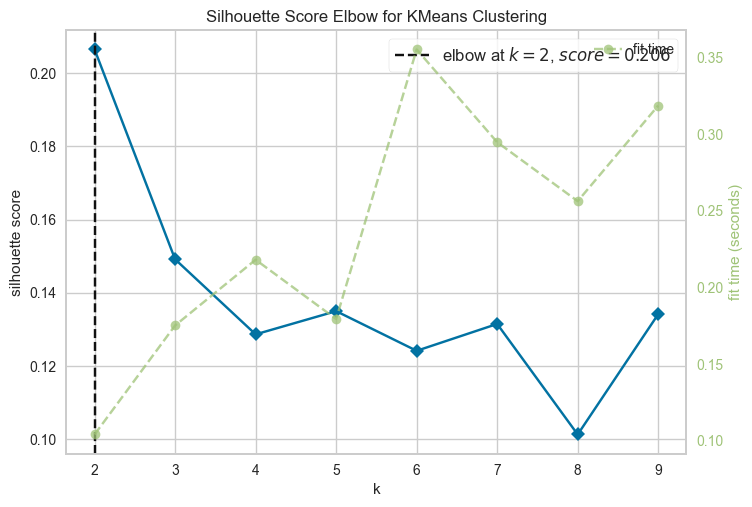
\includegraphics[scale=0.6]{images/ELBO.png}
  \centering
  \caption{ELBO method}
  \label{fig:ELBO}
\end{figure}
As one can see, both the maximum score and fit time are when k=2. 
\subsubsection*{PCA}
Moreover, I decided to use PCA to reduce the dimensionality of the dataset and apply on it the KMeans in order to plot and visualize the data. Furthermore, this allowed me to see if ELBO method was actually correct. 
\begin{figure}[H]
  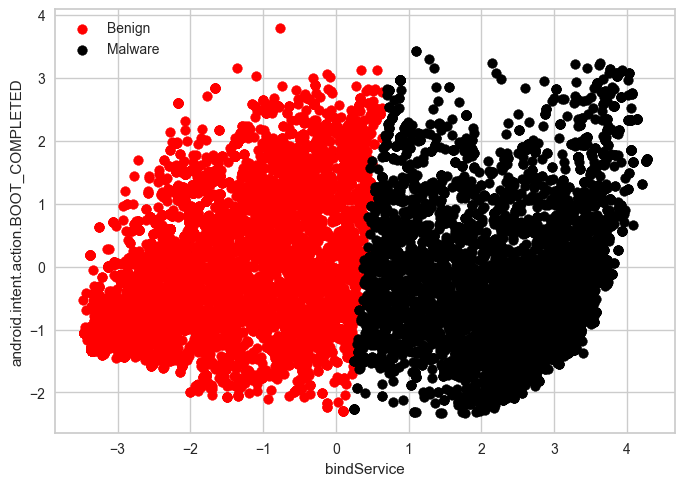
\includegraphics[scale=0.6]{images/PCA.png}
  \centering
  \caption{PCA}
  \label{fig:PCA}
\end{figure}
In fact, the data are almost linearly separable.
\subsubsection*{Preprocessing}
I noticed that some rows on the 92nd column
 of the dataset were filled with \textbf{?}. 
 Obviously, this could be a problem during the 
 training. Consequetly, I replaced these values
  with zeros since I presumed that the values 
  themselves were unknown and the number of these
 occurencies was not crucial for the task. \\
 Moreover, I converted Bs and Ss with 0s and 1s respectively to get a label number representation. \\
 Finally, I report the correlation matrix of the dataset to see which features are more correlated with labels. 

\begin{figure}[H]
  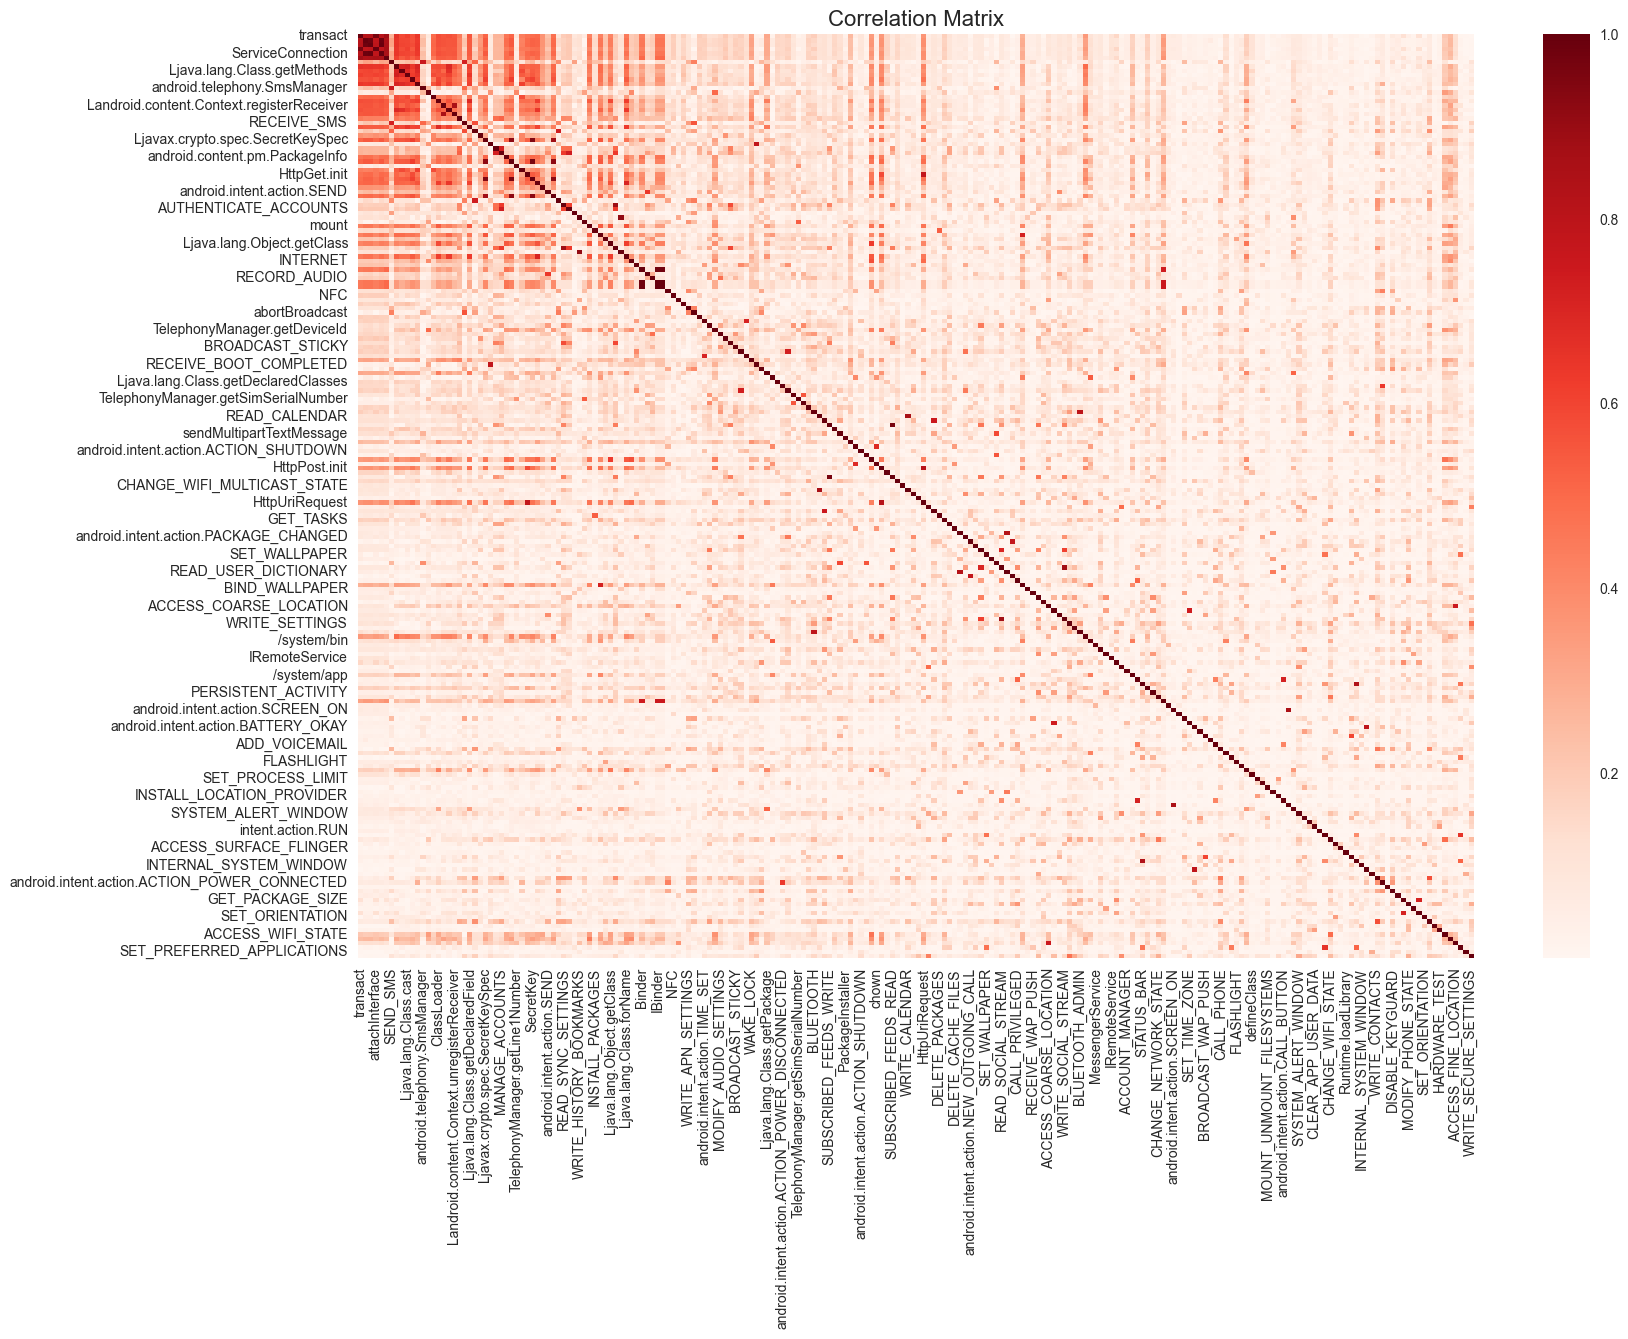
\includegraphics[scale=0.4]{images/CORRMATRIX.png}
  \centering
  \caption{Correlation matrix}
  \label{fig:corr}
\end{figure}
It turns out that the most correlated features are:
'bindService', 'attachInterface', 'ServiceConnection', 'SecretKey', 'IBinder', 'android.os.IBinder', 'SUBSCRIBED\_FEEDS\_READ'\\

\subsubsection*{Data Splitting}
I decided to split the dataset in 3 parts:
\begin{itemize}
  \item Training set: 60 \%
  \item Validation set: 20 \%
  \item Test set: 20 \%
\end{itemize}

\subsubsection*{ML models}
I have chosen 3 models:
\begin{itemize}
  \item Neural Networks: usually works very well for almost every task
  \item Gaussian Naive Bayes: it is a simple model that can be used for binary classification
  \item Decision Tree: simple and easy-readable model
\end{itemize}
In order to find the best hyperparameters (tuning) I wrote a function called \textit{GridSearchFun} which uses GridSearch for searching over specified parameter values for an estimator. In addition, this function returns the best estimator for each model. 
I draw below the NN loss function 
(both training and validation) (fig. \ref{fig:NN}).
\begin{figure}[H]
  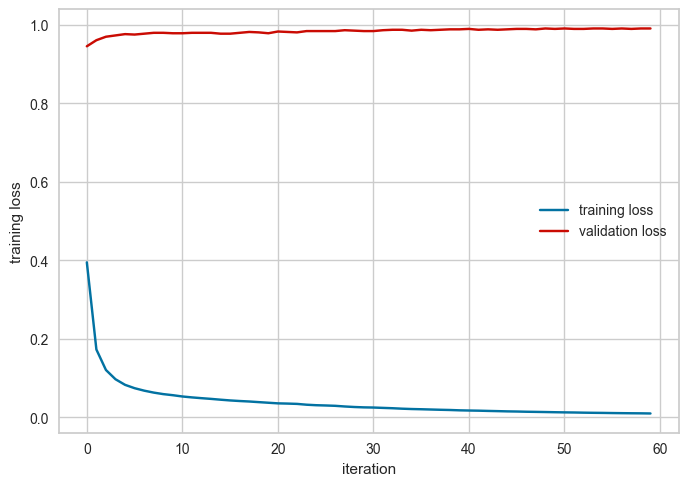
\includegraphics[scale=0.6]{images/NNlossFun.png}
  \centering
  \caption{NN loss function}
  \label{fig:NN}
\end{figure}
Since for Decision Tree and Gaussian NB there is not a training loss I used \textit{learning\_curve} that determines cross-validated training and test scores for different training set sizes. In this way it has been easier to plot and visualize how the models perform during training. \\
The blue line represents the mean of the computed balanced accuracy. Moreover, ShuffleSplit has been used for validation scores through the mentioned sklearn learning curve. Below the final results (fig. \ref{fig:GNBloss} and fig. \ref{fig:DTloss}). 
\begin{figure}[H]
  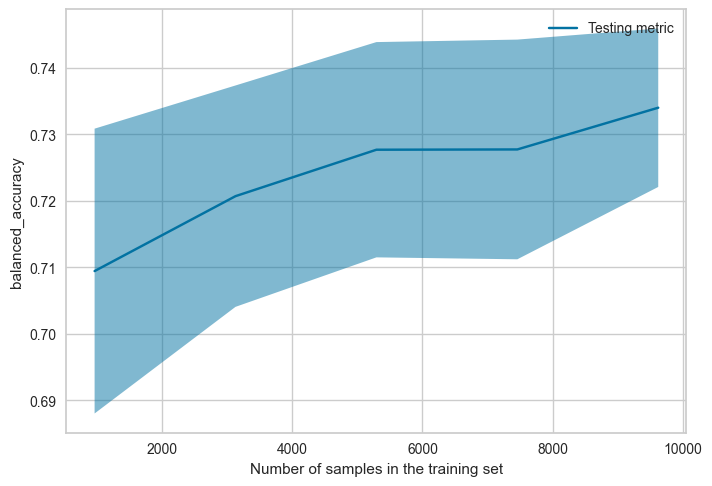
\includegraphics[scale=0.6]{images/GaussianNBtrainingLoss.png}
  \centering
  \caption{Learning Curve Gaussian NB}
  \label{fig:GNBloss}
\end{figure}
\begin{figure}[H]
  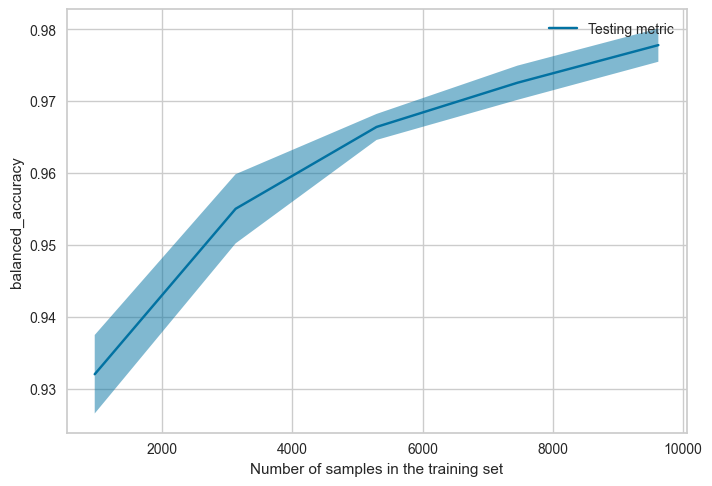
\includegraphics[scale=0.6]{images/DTtrainingLoss.png}
  \centering
  \caption{Learning Curve Decision Tree}
  \label{fig:DTloss}
\end{figure}
As one can see, 
the best model is 
the Decision Tree with a balanced 
accuracy during training of almost 
96\%. However, the NN seems to be the best
 candidate during the testing. In fact, 
 looking at the test phase the NN performs
  very well (tab. \ref{tab:testResults}).
\begin{table}[H]
  \centering
  \begin{tabular}{|l|l|l|}
  \hline
  \textbf{Model}         & \textbf{Balanced Accuracy} & \textbf{Accuracy} \\ \hline
  \textit{NN}            & 0.9851                     & 0.9857            \\ \hline
  \textit{Decision Tree} & 0.9680                     & 0.9697            \\ \hline
  \textit{Gaussian NB}   & 0.7897                     & 0.7446            \\ \hline
  \end{tabular}
  \caption{Test results}
  
  \label{tab:testResults}
  
  \end{table}
Furthermore I plotted the confusion matrix to confirm visually the results I obtained. 
\begin{figure}
  \centering
  \subfloat[Neural Networks]{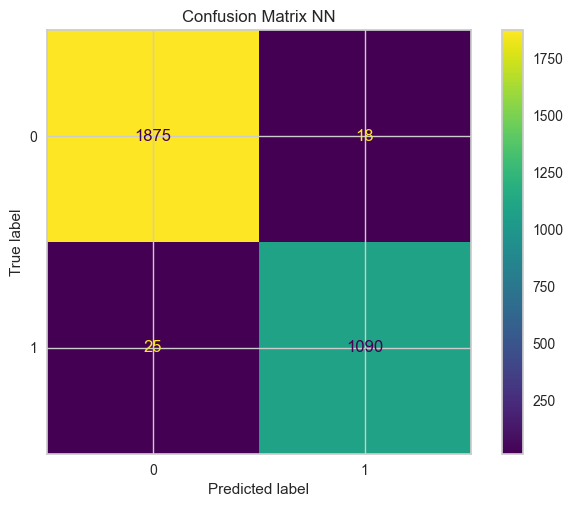
\includegraphics[width=0.3\textwidth]{images/NNCM.png}}\hfill
  \subfloat[Gaussian NB]{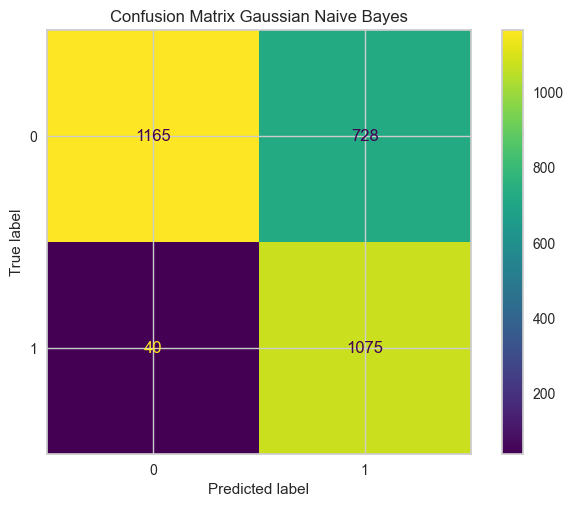
\includegraphics[width=0.3\textwidth]{images/GNBCM.png}}\hfill
  \subfloat[Decision Tree]{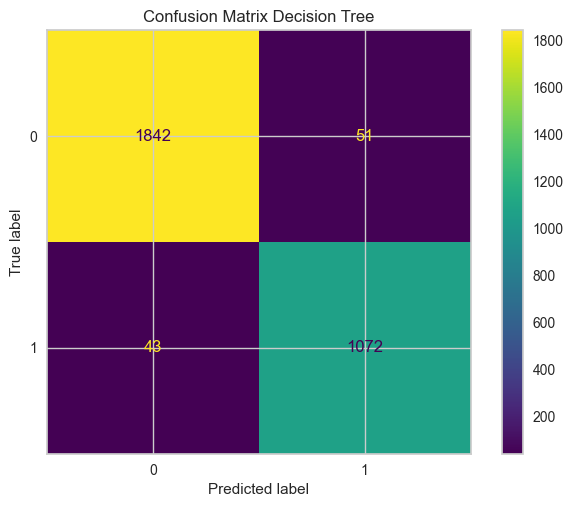
\includegraphics[width=0.3\textwidth]{images/DTCMpng.png}}
  \caption{Confusion Matrix}
\end{figure}
\subsection{Quality of the Dataset}
I believe that the dataset is valuable since both NN and Decision Tree can be considered good models for this task (False Negatives). 
Moreover with a more complex model the results could be much better, maybe reaching almost 100 percent of f1 score and balanced accuracy. 



\subsection{Bypassing your Model}
I picked up the very first sample from the test set. For each model I change every time the probability to swap 0s to 1s each feature of the sample. 
It turns out that the best model that recognizes the sample as malicious is the decision tree. However, the probability to catch it is very low (about 40\% Accuracy). NN performs worse (about 20 \%).\\
I changed 0s to 1s because I wanted to keep the hostile features as they were without compromising the malicious signatures or permissions.  
In the end I successfully bypassed my models. 
\subsection{Improving your Model}
The first thing I have done to improve the results was semplifying the dataset by removing those features that are really correlated with others. \\
Secondly, I used the model SVC (support vector machine for classification). It turns out that it can be very accurate on both the point of the previous exercise and the test set. It reaches a balanced accuracy of more than 97 \%. 
\section{Hardware Trojan Detection}
\end{document}

